%\documentclass{article}           %% ceci est un commentaire (apres le caractere %)
%\usepackage[latin1]{inputenc}     %% adapte le style article aux conventions francophones
%\usepackage[T1]{fontenc}          %% permet d'utiliser les caract�res accentu�s
%\usepackage[dvips]{graphicx}      %% permet d'importer des graphiques au format .EPS (postscript)
%\usepackage{fancybox}		   %% package utiliser pour avoir un encadr� 3D des images
%\usepackage{makeidx}              %% permet de g�n�rer un index automatiquement


\documentclass{article}[12pt]
\usepackage[left=1.5cm,right=1.5cm,top=1.5cm,bottom=2cm]{geometry} % page settings
\usepackage{amsmath} % provides many mathematical environments & tools
\usepackage{indentfirst}
\setlength{\parindent}{24pt}
%\setlength{\baselineskip}{1cm}
%\parskip = \baselineskip
%\parskip = 1cm 
%\setlength{\parskip}{1cm}
%\usepackage[parfill]{parskip}

\setlength{\parindent}{4em}
\setlength{\parskip}{1em}
\renewcommand{\baselinestretch}{1.1}


\usepackage[T1]{fontenc} % Use 8-bit encoding that has 256 glyphs
\usepackage[utf8]{inputenc} % Required for including letters with accents
\usepackage{graphicx} % Required for including images
\graphicspath{{figures/}} % Set the default folder for images


\usepackage{enumitem} % Required for manipulating the whitespace between and within lists
\usepackage{lipsum} % Used for inserting dummy 'Lorem ipsum' text into the template
%\usepackage{subfig} % Required for creating figures with multiple parts (subfigures)
\usepackage{subcaption}
\usepackage{amsmath,amssymb,amsthm} % For including math equations, theorems, symbols, etc
\usepackage[toc]{appendix}

\usepackage{tikz}
\usepackage{pgfplots}




%\usepackage{pst-func}
%\pgfplotsset{compat=newest}

%\directlua{
%  ffi=require("ffi")
%  ffi.cdef[[
%  double jn(int n, double x);
%  double yn(int n, double x);
%  ]]
%}

%\pgfmathdeclarefunction{BesselJ}{2}{%
%  \edef\pgfmathresult{%
%    \directlua{tex.print(ffi.C.jn(\pgfmathfloatvalueof{#1},%\pgfmathfloatvalueof{#2}))}%
%  }%
%}

%\pgfmathdeclarefunction{BesselY}{2}{%
%  \edef\pgfmathresult{%
%    \directlua{tex.print(ffi.C.yn(\pgfmathfloatvalueof{#1},%\pgfmathfloatvalueof{#2}))}%
%  }%
%}





\graphicspath{{figures/}} % Set the default folder for images
\setlength{\parindent}{0mm}
\usepackage{hyperref}

\title{Atmospheric Monitoring}     %% \title est une macro, entre { } figure son premier argument
\author{Sylvie Dagoret-Campagne, Marc Moniez}        %% idem

\makeindex		    %% macro qui permet de g�n�rer l'index
\bibliographystyle{prsty}	  %% le style utilis� pour cr�er la bibliographie
\begin{document}                  %% signale le d�but du document



\maketitle                        %% produire � cet endroit le titre de l'article � partir des informations fournies ci-dessus (title, author)
%\newpage
%\tableofcontents                  %% produire � cet endroit la table des mati�ree				

\section{Introduction}	

The usual approach in photometric calibration in a filter band $b$ is presented in this section.
Let us consider an object above the atmosphere with a specific flux\footnote{A specific flux is usually expressed in Jansky unit where 1Jy=$1~erg/s/cm^2/Hz$.} $F_\nu(\lambda)$.
Its flux at telescope pupil $F_\nu(\lambda,t)^{pupil}(\lambda,az,alt,t)$ (before entering the telescope) is~:
\begin{equation}
F_\nu(\lambda,t)^{pupil}(\lambda,az,alt,t) = T_{atm}(\lambda,az,alt,t)\cdot F_\nu(\lambda)
\end{equation}
where $T_{atm}(\lambda,az,alt,t)$ is the atmospheric transmission which has the following form:
\begin{equation}
T_{atm}(\lambda,az,alt,t) = e^{-\tau(\lambda,az,alt,t)}
\end{equation}

The flux is observed through a passband $b$ of the telescope and an ADU\footnote{ADU means ADC units.} counting rate $C_b$ is recorded by the CCD after conversion of the photons into photoelectrons in the pixel of coordinates $(x,y)$ :
\begin{equation}
C_b(alt,az,t,x,y) = C \int F_\nu^{pupil}(\lambda,az,alt,t)\cdot S^{syst}_b(\lambda,t,x,y) \frac{d\lambda}{\lambda}  
\end{equation}
where the $1/\lambda$ comes for the conversion of energy into a photon.

The constant $C$ is~:
\begin{equation}
C = \frac{\pi D^2}{4 g h}
\end{equation}
where $g$ is the electronic conversion of the number of photoelectrons per ADU count ($g>1$).

Le us defines the effective normalised passband $\Phi^{obs}(\lambda,t)$~:

\begin{equation}
\boxed{
\Phi^{obs}_b(\lambda,t) = \frac{T_{atm}(\lambda,az,alt,t)\cdot S^{syst}_b(\lambda,t,x,y) \cdot \frac{1}{\lambda}}{\int_b T_{atm}(\lambda,az,alt,t)\cdot S^{syst}_b(\lambda,t,x,y) \frac{d\lambda}{\lambda}}
}
\end{equation}
Note above the $(x,y)$ pixel variation should have been corrected.
Then
\begin{equation}
\int_b \Phi^{obs}_b(\lambda,t) d\lambda =1
\end{equation}

Note any grey attenuation component in the atmospheric transmission is removed in the definition of $\Phi^{obs}_b(\lambda,t)$.

The observed flux $F_b^{obs}(t)$ in the band $b$ reads:
\begin{equation}
F_b^{obs}(t)= \int F_\nu(\lambda) \Phi^{obs}_b(\lambda,t) d\lambda \propto C_b(alt,az,t)
\end{equation}


Even if the source has a steady flux $F_\nu(\lambda)$, $F_b^{obs}(t)$ varies in time due to atmospheric variation (even one could include instrument non-corrected variation).
However in a catalogue we should report a constant value independent of atmospheric condition. 

Thus one should provide a standardized flux $F_b^{std}$ observed through a standardized effective normalized passband $\Phi^{std}_b(\lambda)$~:
\begin{equation}
F_b^{std}= \int F_\nu(\lambda) \Phi^{std}_b(\lambda) d\lambda
\end{equation}



The flux are given in "natural" magnitude unit~:
\begin{equation}
m^{nat}_b = -2.5 \log_{10}\left( \frac{F_b^{obs}}{F_{AB}} \right)
\end{equation}
where the observed flux is reported relative to an unobserved ideal $AB$ source through the same similar effective filter.

An ideal $AB$ source is $F_\nu(\lambda) = 3631 Jy$.

The natural magnitudes can be translated into a standardized magnitudes as follow~:

\begin{eqnarray}
m^{nat}_b & = & -2.5 \log_{10}\left( \frac{F_b^{obs}}{F_{AB}}\right) \\
& = & -2.5 \log_{10}\left( \frac{\int F_\nu(\lambda) \Phi^{obs}_b(\lambda,t) d\lambda}{F_{AB}}\right) 
\\
& = & -2.5 \log_{10}\left( \frac{\int F_\nu(\lambda) \Phi^{obs}_b(\lambda,t) d\lambda}{\int F_\nu(\lambda) \Phi^{std}_b(\lambda) d\lambda}\right) 
-2.5 \log_{10}\left( \frac{\int F_\nu(\lambda) \Phi^{std}_b(\lambda) d\lambda}{F_{AB}}\right)
\end{eqnarray}

\begin{equation}
m^{nat}_b = \Delta m^{obs}_b + m^{std}_b
\end{equation}

where the ratio
\begin{equation}
\boxed{
\Delta m^{obs}_b  = -2.5 \log_{10}\left( \frac{\int F_\nu(\lambda) \Phi^{obs}_b(\lambda,t) d\lambda}{\int F_\nu(\lambda) \Phi^{std}_b(\lambda) d\lambda}\right) 
}
\end{equation}
which depends on the wavelength dependence of $F_\nu(\lambda)$ is a calibration factor.

$m^{std}_b$ is the magnitude to be quoted in the catalog in addition to $ \Phi^{std}_b(\lambda)$. Then magnitudes between experiment can be compared and even translated in another magnitude unit.

In general, a standard calibration procedure consists in giving the standardized magnitude or measured objects:
\begin{equation}
\boxed{
m^{std}_b = -2.5 \log_{10} (C_b(alt,az,t)) - \Delta m^{obs}_b + Z_b(t)
}
\end{equation}

where:
\begin{itemize}
\item $C_b(alt,az,t)$ is the measured experimentally measured in ADU unit,
\item $\Delta m^{obs}_b$ is the color correction in that band for that particular object with a particular wavelength dependence $F_\nu(\lambda)$, (not including any grey - flat wavelength attenuation),
\item $Z_b$ is defined as the zero point includes correction wavelength independent that are similar for all sources observed in the field of view of the telescope at the same time.
\end{itemize}

$Z_b$ in addition to the time varying grey attenuation, the zero point includes constants related to the definition of the reference system, here the $AB$ source reference. 


\begin{equation}
\boxed{
Z_b^{obs}(t) = 2.5 \log_{10}\left( C F_{AB} \int_0^\infty S^{atm}(\lambda,alt,az,t) S^{syst}_b(\lambda,x,y,t) \frac{d\lambda}{\lambda}\right)
}
\end{equation}


\section{Method}

In the following method, we develop at first order the wavelength dependence of the SED and also the atmospheric transmission wavelength dependence.

Let us define for some reference time $t_0$~:

\begin{itemize}
\item ${\cal F}_S(\lambda, t_0) \simeq {\cal F}_S(\lambda)$ the Spectral Energy Distribution (SED) of some reference star supposed to be steady in Luminosity (in units of photons or photoelectrons per wavelength unit),

\item $T(\lambda,\hat{z},t_0)$ the atmospheric transmission at airmass $\hat{z}$ corresponding at Auxtel pointing at time $t_0$, which is the quantity we want to monitor,

\item $I_V(\lambda,t_0)$, the total instrumental transmission supposed to be constant or corrected such~:
\begin{equation}
I_V(\lambda,t_0) = V(\lambda,t_0) \cdot \epsilon_{CCD}(\lambda,t_0) \cdot  O(\lambda,t_0)
\end{equation} 
where $ V(\lambda,t_0)$ is the filter passband (ex. the LSST Filter band : V= U,G,R,I,Z,Y), $\epsilon_{CCD}(\lambda,t_0) $ is the quantum efficiency, $O(\lambda,t_0)$ is the optical throughput. 
\end{itemize}

We define the varying function~:
\begin{equation}
{\cal \tau} (\lambda,t) = T(\lambda,\hat{z},t) \cdot I_V(\lambda,t)
\end{equation}


The reference spectrum $S_V(t_0)$ measured in the telescope at reference time $t_0$ is~:

\begin{equation}
S_V(t_0) = A \int_V {\cal F}_S(\lambda, t_0) T(\lambda,\hat{z},t_0)  I_V(\lambda,t_0) d\lambda
\end{equation}
where $A$ is an known constant.

We can rewrite the measured spectrum $S_V(t)$ at any time $t$ in a more compact form~:
\begin{equation}
S_V(t) = A \int_V {\cal F}_S(\lambda){\cal \tau}(\lambda, t)d\lambda
\label{eq:refspectrum}
\end{equation} 

We assume an ideal AB source which spectrum is fully defined  
${\cal F}_{AB}$.

For that particular ideal source, let us define the following ratio~:

\begin{equation}
k(t) = \frac{\int{\cal \tau}(\lambda,t ) {\cal F}_{AB}d \lambda }{\int{\cal \tau}(\lambda,t_0) {\cal F}_{AB}d \lambda}
\end{equation}


$k(t)$ encapsulate time dependence of grey attenuation.
Let us assume this $k(t)$ to be fully estimated.


Let us defines the grey attenuation corrected quantities~:
\begin{equation}
\left\{
\begin{array}{ccc}
S^\prime_V(t) & = & \frac{S_V(t)}{k(t)} \\
{\cal \tau}^\prime(\lambda, t) & = & \frac{{\cal \tau}(\lambda,t)}{k(t)} \\
\end{array}
\right.
\end{equation}

Then observing a reference star S of flux ${\cal F}_S$ for which
the equation~\ref{eq:refspectrum} is well established at time $t_0$.



\begin{equation}
\frac{S_V^\prime(t) - S_V(t_0)}{S_V(t_0)} =  \frac{A}{S_V(t_0)} 
\int_V \left( {\cal \tau}^\prime(\lambda, t) - {\cal \tau}(\lambda, t_0) \right) {\cal F}_S(\lambda) d\lambda 
\end{equation}
 

Because we know quite well the flux of the reference star in the V band, we assume we can approximate  ${\cal F}_S(\lambda)$ at first order in the band $V$ with $\lambda_V$ is the V-band center as follow:


\begin{equation}
{\cal F}_S(\lambda)|_V = {\cal F}_{AB}(\lambda_V) \left(1+ \alpha_S(\lambda - \lambda_V)\right)
\end{equation}

\begin{equation}
\frac{S_V^\prime(t) - S_V(t_0)}{S_V(t_0)} =  \frac{A}{S_V(t_0)} \int_V \left( {\cal \tau}^\prime(\lambda, t) - {\cal \tau}(\lambda, t_0) \right) {\cal F}_{AB}(\lambda_V) \left(1+ \alpha_S(\lambda - \lambda_V)\right) d\lambda
\end{equation}


We make a second assumption\footnote{I don't understand this approximation is true.} :
\begin{equation}
{\cal \tau}^\prime(\lambda, t) - {\cal \tau}(\lambda, t_0)  = {\cal \tau}(\lambda, t_0)\left(\frac{1}{k(t)}\frac{{\cal \tau}(\lambda,t) }{{\cal \tau}(\lambda,t_0)} -1 \right) \simeq {\cal \tau}(\lambda, t_0) a(t) (\lambda-\lambda_V)
\end{equation}


\begin{figure}
    \centering
    \begin{subfigure}{0.99\textwidth}
        \centering
        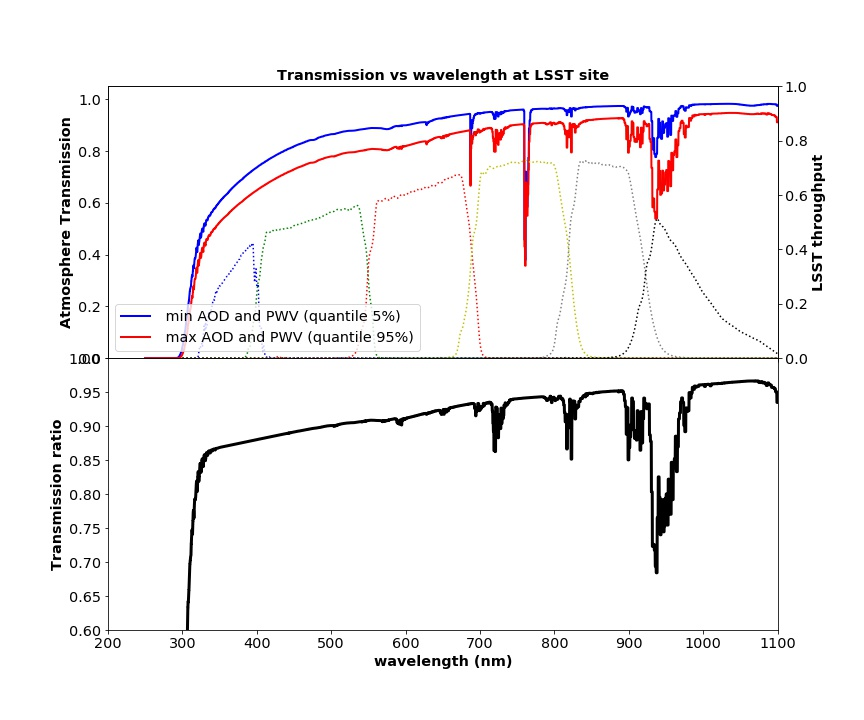
\includegraphics[width=16cm]{figures/AtmTransparency_LSST_AER_PWV_ratio.jpg}
        \caption{Quantiles of the atmospheric transmission profile and their ratio.}
    \end{subfigure}%
\end{figure}



The Magnitude variation of the source S in the V band is:
\begin{equation}
dM^S_{V_{AB}} = -\frac{2.5}{\ln(10)} \frac{dF^S_{V_{AB}}}{F_{V_{AB}}}
\end{equation}

Then 
\begin{equation}
-\frac{\ln(10)}{2.5} \left(M^S_{V_{AB}}(t)- M^S_{V_{AB}}(t_0) \right) \simeq
\frac{A {\cal F}_{AB}(\lambda_V)  {\cal \tau}(\lambda, t_0) }{S_V(t_0)}a(t)\int_{\lambda_V-\Delta \lambda/2}^{\lambda_V+\Delta \lambda/2}(\lambda- \lambda_V)\left(1+ \alpha_S(\lambda - \lambda_V)\right) d\lambda
\end{equation}

We defines $\Delta \lambda$:
\begin{equation}
\Delta \lambda = \frac{S_V(t_0)}{A {\cal F}_{AB}(\lambda_V)  {\cal \tau}(\lambda, t_0)} 
\end{equation}

\begin{equation}
0.921 \left(M^S_{V_{AB}}(t)- M^S_{V_{AB}}(t_0) \right) = \frac{a(t) \alpha_S}{12}(\Delta \lambda)^2
\end{equation}

%%%%%%%%%%%%%%%%%%%%%%%%%%%%%%%%%%%%%%%%%%%%%%%%%%%%%%%%%%%%%%%%%%%%%%%%%%%%%%%%

\newpage
\appendix 

\section*{Appendix}

\section{\\Magnitudes in AB system}

The flux reference in a AB system is the flat SED in Jansky units such~:

\begin{equation}
{\cal{F}}_\nu^{E} = \frac{d P}{d\nu dS}  = 3631 Jy
\end{equation}

where $dP= \frac{dE}{dt}$ is the power emitted by the source and $\nu$ the frequency and $dS$ a surface element.

\begin{equation}
   1 Jy = 10^{-26} W \cdot Hz^{-1} \cdot m^{-2} = 10^{-23} erg \cdot s^{-1} \cdot Hz^{-1} \cdot cm^{-2} 
\end{equation}

The energy, frequency and wavelength are related by:
\begin{equation}
E=h \nu = \frac{h c}{\lambda}
\end{equation}

Given that

\begin{equation}
\frac{dP}{dS} = {\cal{F}}_\nu^{E} d\nu = {\cal{F}}_\lambda^{E} d\lambda 
\end{equation}

\begin{equation}
{\cal{F}}_\lambda^{E} = {\cal{F}}_\nu^{E} \frac{d\nu}{d \lambda} = \frac{c}{\lambda^2} {\cal{F}}_\nu^{E}
\end{equation}



To convert this power $dP$  into a number a photon rate $dn_\gamma$~:
\begin{equation}
\frac{d n_\gamma}{dS} = \frac{\lambda}{hc} \frac{dP}{dS}
\end{equation}


Then the photon flux ${\cal F}^{n_\gamma}_\lambda$ is given by


\begin{equation}
\frac{dn_\gamma}{dS}={\cal F}^{n_\gamma}_\lambda d\lambda = \frac{d n_\gamma}{dP} {\cal F}^{E}_\lambda d\lambda = \frac{\lambda}{hc} \frac{c}{\lambda^2} {\cal F}^{E}_\nu d\lambda
\end{equation}

Finally

\begin{equation}
{\cal F}^{n_\gamma}_\lambda = \frac{1}{h\lambda}{\cal F}^{E}_\nu 
\end{equation}

The SED for an ideal perfect AB source is,
\begin{eqnarray}
{\cal F}^{n_\gamma}_{\lambda AB} & = &\frac{3631 Jy}{h\lambda} = 
\frac{3631 \times 10^{-26} W/Hz /m^2 \times 10^{-4} m^2/cm^2}{6.26\cdot 10^{-34} J.s /550 nm}
\left( \frac{550 nm}{\lambda_{nm}} \right) \\
& = & 9972~phot/s/nm/cm^2 \left( \frac{550 nm}{\lambda_{nm}} \right)
\end{eqnarray}

It has an $1/\lambda$ photon distribution.



\section{\\Approximation of a source flux in a band filter}

\subsection{Power law}
Let us assume in a band $V$ width the Flux of a star  ${\cal F}_S(\lambda)$ can be approximated at first order by a power law if index $\alpha_S$ as follow~:
\begin{equation}
{\cal F}_S(\lambda) \simeq {\cal F}_S(\lambda_V) (\lambda-\lambda_V)^{\alpha_S}
\end{equation}

This expression can be developed as follow~:

\begin{eqnarray}
{\cal F}_S(\lambda) & \simeq &  {\cal F}_S(\lambda_V) + \left( \frac{d {\cal F}_S }{d\lambda}\right)({\lambda_V})(\lambda-\lambda_V) \\
& \simeq & {\cal F}_S(\lambda_V) \alpha_S (\lambda-\lambda_V)
\end{eqnarray}

\subsection{Exponential Law}
If the flux is expressed as~:

\begin{equation}
{\cal F}_S(\lambda) \simeq {\cal F}_S(\lambda_V)  e^{\alpha_S (\lambda-\lambda_V)} 
\end{equation}

then we still have the same approximation at first order:

\begin{eqnarray}
{\cal F}_S(\lambda) & \simeq &  {\cal F}_S(\lambda_V) + \left( \frac{d {\cal F}_S }{d\lambda}\right)({\lambda_V})(\lambda-\lambda_V) \\
& \simeq & {\cal F}_S(\lambda_V) \alpha_S (\lambda-\lambda_V)
\end{eqnarray}



\section{Function ${\cal \tau}(\lambda,t)$}

\begin{equation}
{\cal \tau}^\prime(\lambda, t) - {\cal \tau}(\lambda, t_0)  = {\cal \tau}(\lambda, t_0)\left(\frac{1}{k(t)}\frac{{\cal \tau}(\lambda,t) }{{\cal \tau}(\lambda,t_0)} -1 \right) = {\cal \tau}(\lambda, t_0) \left(\frac{T(\lambda,t)}{T(\lambda,t_0)}-1   \right)
\end{equation}

The atmospheric transmission can be parametrized as~:

\begin{equation}
T(\lambda,t,z) = \exp( -K(\lambda,t)z)
\end{equation}

$K(\lambda,t)$ is the atmospheric extinction coefficient.

\begin{equation}
K(\lambda,t) = \frac{K_r^{scatt}(t)}{\lambda^4} + \frac{K_a^{scatt}(t)}{\lambda^{\beta(t)}} + \sum_i K_i^{abs}(\lambda)a_i(t)
\end{equation}

\begin{itemize}
\item $\frac{K_r^{scatt}(t)}{\lambda^4}$ is the extinction coefficient for Rayleigh, where $K_r^{scatt}(t) = K_r^{scatt}(t_0)\frac{P(t)}{P(t_0)} $ scattering,
\item $\frac{K_a^{scatt}(t)}{\lambda^{\beta(t)}}$ is the extinction coefficient for aerosol scattering,
\item $K_i^{abs}(\lambda)a_i(t)$ is the extinction coefficient for molecular absorption of $O_2, O_3$ and precipitable water vapor. 
\end{itemize}

For all interaction processes, the wavelength part is separated from the time dependant part except for the aerosols for which the exponent depends on time. 

The Rayleigh contribution is supposed perfectly known because the pressure $P(t)$ is measured and the absorption band $K_i^{abs}$ is constant and known.
The varying parameters, the aerosol parameters $K_a^{scatt}(t), \beta(t)$, the absorption coefficient $a_i(t)$\footnote{$a_i(t)$ for Ozone will be monitored by Satellite data} for PWV require to be monitored.

If atmospheric variations are small enough,
\begin{eqnarray}
R(\lambda,t)& = &\frac{T(\lambda,t,z)}{T(\lambda,t_0,z)}-1 = \exp\left\{-\left(K(\lambda,t)- K(\lambda,t_0) \right)z-1\right\}
\\ &  \simeq & \left(K(\lambda,t)- K(\lambda,t_0) \right)z
\end{eqnarray}

In a band $V$, $K(\lambda,t)$ can be expressed at first order as~:

\begin{equation}
K(\lambda,t) = K(\lambda_V,t) + \frac{\partial K}{\partial \lambda}_{\lambda=\lambda_V}(\lambda-\lambda_V)
\end{equation}

If $K \simeq \frac{K_0}{\lambda^\delta}$,  $\frac{\partial K}{\partial \lambda} \simeq - \delta \frac{K_0}{\lambda^{\delta+1}} \simeq - \delta \frac{K}{\lambda}$

\begin{itemize}
\item For Rayleigh scattering , $K_r^{scatt}(\lambda,t)= K_r^{scatt}(\lambda_V,t)(1-4\frac{\lambda-\lambda_V}{\lambda_V})$,
\item For Aerosols, $K_a^{scatt}(\lambda,t)= K_a^{scatt}(\lambda_V,t)(1-\beta(t)\frac{\lambda-\lambda_V}{\lambda_V})$,
\end{itemize}

We do not develop the $K_i^{abs}(\lambda)$ with respect to $\lambda=\lambda_V$, because the $K_i^{abs}(\lambda)$ quickly vary with $\lambda$ within the wavelength band. This contribution will be absorbed in the in band constant $a_i(t)$. 

\begin{eqnarray}
\frac{R(\lambda,t)}{z}& = & \left( K_r^{scatt}(\lambda_V,t) - K_r^{scatt}(\lambda_V,t_0) \right) (1-4\frac{\lambda-\lambda_V}{\lambda_V}) \\
& + & \left( K_a^{scatt}(\lambda_V,t) - K_a^{scatt}(\lambda_V,t_0)\right) - (K_a^{scatt}(\lambda_V,t_0)(\left( \beta(t) -\beta(t_0)\right)\frac{\lambda-\lambda_V}{\lambda_V}) \\
& + & \sum_i \overline {K_i^{abs}}\left(a_i(t)-a_i(t_0) \right)
\end{eqnarray}

This term may be written in a compact form~:
\begin{equation}
\frac{R(\lambda,t)}{z} =  K_r^0 \frac{\delta P(t)}{P} (1-4\frac{\lambda-\lambda_V}{\lambda_V}) 
 +  \Delta K_a(t) - K_a^0 \Delta \beta(t) \frac{\lambda-\lambda_V}{\lambda_V} 
 +  \sum_i \overline {K_i^{abs}} \Delta a_i(t)
\end{equation}

We can even simplify this equation~:
\begin{equation}
\frac{R(\lambda,t)}{z} = A(t) + B(t) \frac{\lambda-\lambda_V}{\lambda_V} + \sum_i C_i^{abs}(t)
\end{equation}

The expression above show color neutral terms and color dependant terms (weighted by $\frac{\lambda-\lambda_V}{\lambda_V}$).

The monitoring variables to estimate from AuxTel data are $A_V(t), B_V(t), C_{iV}^{abs}(t)$.

The $A(t)$ term may be absorbed when subtracting the grey component.But this grey component is present in the Rayleigh and Aerosol simulation.
$B(t)$ may be present in all bands.
$C_{O^3}$ is present in G and R band, $C_{O^2}$ in I band (may be also some $C_{H2O}$ in I band), and $C_{PWV}$ in Y band.


\newpage

\section{Old personal notes}

\subsection{Spectral Energy Distribution}
%-----------------------------------------------

The spectrum is a Spectral Energy Density (SED) written as $S_{\lambda}^{E}(\lambda)$ (The E in the superscript refers to the energy or power distribution which is not the number of photons distribution).
For example for the CALSPEC database, the spectra unit is and ${\rm erg.s^{-1}. cm^{-2} \AA^{-1}}$ , the wavelength is in  given Angstroms(\AA). 


\subsection{Measurement}
%---------------------------

However the CCD make some measurement of the number of photo-electrons $n_{e}(\lambda)d\lambda$ (number of photo-electrons per second in $d\lambda$ unit wavelength)
or number of photons $n_{\gamma}(\lambda)d\lambda$ (number of photons per second in $d\lambda$ unit wavelength).

The relation between the number of electrons $d N_{e} =  n_{e}(\lambda) \cdot d\lambda$, the number of photons  $ dN_{\gamma} =  n_{\gamma}(\lambda) \cdot d\lambda$ and the ADU count numbers $dN_{ADU} =  n_{ADU}(\lambda) \cdot d\lambda$ (CCD signal digitization units) in wavelength unit $d\lambda$ per unit of time $dt$ (one second) is:

$$
d N_{e}  = n_{e}(\lambda) \cdot d\lambda =\epsilon_{CCD}(\lambda)\cdot n_{\gamma}(\lambda) \cdot d\lambda = g_{el} \cdot n_{ADU}(\lambda) \cdot d\lambda
$$

where
\begin{itemize}
\item $\epsilon_{CCD}(\lambda)$ : CCD quantum efficiency, no unit,
\item $g_{el}$ : electronic gain used to convert ADU into electrons, it is in unit of electron per ADU,
\item $n_{e}(\lambda)$ : number of electrons in a pixel per wavelength unit $d\lambda$ and per time unit $dt$,
\item $S_{\lambda}^{E}(\lambda)$ : SED : energy per wavelength unit, collection surface unit, detection time unit (exposure), and wavelength unit (in present CALSEC case, erg per cm$^2$ per second per Angstrom). 
\end{itemize}

\subsection{Spectrum in photon unit}

The CCD measures a number of photons that induce photoelectrons, not the incident energy. Thus we have to convert
the spectral energy density of the source $S^E_{\lambda} (\lambda) \cdot d\lambda$ into a number of photon energy density
$S^{N_\gamma}_{\lambda}(\lambda) \cdot d\lambda$ :

$$
S^{N_\gamma}_{\lambda} (\lambda) \cdot d\lambda = \frac{S^E_{\lambda}(\lambda) \cdot d\lambda}{hc/\lambda}
$$

- The number of photons density from the source is then expressed as $dN_{\gamma}(\lambda)/d\lambda$ :

$$
\frac{dN_{\gamma}(\lambda)}{d\lambda} = S^{N_\gamma}_{\lambda}(\lambda) = \frac{\lambda }{hc} \cdot S^E_{\lambda} (\lambda)
$$


- Note in some textbook, the spectral energy density $S^{E}_\nu (\nu)$ is tabulated in frequency unit.

Given 
$$ dE = S^{E}_\nu (\nu) \cdot d\nu  =   S^{E}_\lambda (\lambda) \cdot d\lambda
$$

$$
S^{E}_\lambda (\lambda) = S^{E}_\nu (\nu) \cdot | \frac{d\nu}{d\lambda} | = \frac{c}{\lambda^2} \cdot S^{E}_\nu (\nu)
$$

thus we can also find the expression for the number of photons in the detector:

$$
\frac{dN_{\gamma}(\lambda)}{d\lambda} = \frac{1 }{h \lambda} \cdot S^E_{\nu} (\nu(\lambda))
$$

Or if we wanted to express $dN_{\gamma}(\lambda)$ as a function of $\nu$ :

$$
dN_{\gamma}(\nu) = dN_{\gamma}(\lambda)\cdot |\frac{d\lambda}{d\nu}|= \frac{c}{\nu^2}\cdot dN_{\gamma}(\lambda)
$$



... to be continued to show:


\subsection{The flux in a wavelength bandwidth}
%---------------------------------------------------------

Transmission in atmosphere $T^{atm}(\lambda)$ , detector filters $T^{filt}(\lambda)$, or grating $T^{grat}(\lambda)$,  optics (mirrors and lenses) $T^{opt}(\lambda)$, detector (CCD) $\epsilon_{CCD}(\lambda)$, focusing efficiency $\epsilon_{PSF}$ are often expressed as a function of the wavelength $\lambda$ and the SED either using $S^{E}_\lambda(\lambda)$ or using $S^{E}_\nu(\nu(\lambda))$: 
( $T^{grat}(\lambda)$ is for auxiliary telescope.)
The flux (in ADU) in a pixel in $\Delta \lambda$ is expressed as:

\begin{eqnarray}
F_{\Delta \lambda}^{ADU}&  =& \frac{\pi D^2}{4 g_{el}} \int_{\Delta \lambda}  T^{atm}(\lambda) \cdot T^{grat}(\lambda) \cdot T^{opt}(\lambda)\cdot T^{filt}(\lambda) \cdot \epsilon_{PSF} \cdot \epsilon_{CCD}(\lambda) \cdot \frac{dN_{\gamma} (\lambda)}{d\lambda} \cdot d\lambda \\
F_{\Delta \lambda}^{ADU} &= &\frac{\pi D^2}{4 g_{el} h c} \int_{\Delta \lambda}  T^{atm}(\lambda) \cdot T^{grat}(\lambda) \cdot T^{opt}(\lambda) \cdot T^{filt}(\lambda)\cdot \epsilon_{PSF} \cdot \epsilon_{CCD}(\lambda) \cdot  S^{E}_\lambda(\lambda)    \cdot \lambda \cdot d\lambda \\
F_{\Delta \lambda}^{ADU} & = &\frac{\pi D^2}{4 g_{el} h} \int_{\Delta \lambda}  T^{atm}(\lambda) \cdot T^{grat}(\lambda) \cdot T^{opt}(\lambda) \cdot T^{filt}(\lambda)\cdot \epsilon_{PSF} \cdot \epsilon_{CCD}(\lambda) \cdot  S^{E}_\nu(\lambda)   \cdot \frac{d\lambda}{\lambda} \\
\end{eqnarray}

\begin{itemize}
\item we should not forget the $\lambda$ term,
\item we should not forget the $T^{grat}(\lambda)$ term. I would guess the following approximation $T^{grat}(\lambda)\propto 1/\lambda^\alpha$ ($\alpha$ is an unknown index power) and that the term $\lambda \cdot T^{grat}(\lambda)$ is quite constant from 600 nm to 1000 nm in our case.
\item $\epsilon_{PSF}$ : Is the fraction of light selected by the aperture. Because the light of a punctual object is spread over the PSF  (standing for Point Spread Function), the aperture may be smaller than the whole extend of the PSF. So $\epsilon_{PSF}<1$
must be known.
\end{itemize}


\subsection{Application to LSST}

LSST measures the flux $F^{ADU}_{filt}$ independently into six filters $F$, where $F=U,G,R,I,Z,Y4$. Each Filter is a passband of transmission function $T_F(\lambda)$. We skip $^{grat}(\lambda) $ and $\epsilon_{PSF}$ for simplicity.
The following table summarise how the Magnitude $M_{filt}$ is computed.


\fbox{\parbox{\textwidth}{
\begin{equation}
F_{filt}^{ADU}(code) = \frac{\pi D^2}{4 g_{el} h c} \int_{\lambda.in.filt}  T^{atm}_{code}(\lambda) \cdot  T^{opt}(\lambda) \cdot T^{filt}(\lambda) \cdot \epsilon_{CCD}(\lambda) \cdot  S^{E}_\lambda(\lambda)    \cdot \lambda \cdot d\lambda \nonumber
\end{equation}
\begin{center}
\begin{tabular}{l c c} \\
$F_{filt}^{ADU}$ & :  & Flux measured in LSST Filter "filt" \\
$ T^{atm}_{code}(\lambda)$ & : & Atmospheric transparency either from Modtran ($code=MT$) or LibRadTran ($code=RT$) \\
$ T^{opt}(\lambda$  & : &Optical througput \\
$T^{filt}(\lambda)$ & : & Filter transmission \\
$\epsilon_{CCD}(\lambda)$ & : & Quantum efficiency of the CCD \\
$S^{E}_\lambda(\lambda)$ & : & SED of astrophysical object \\
$g_{el}$ & : &Electronic gain : number of electrons per ADU \\
$D$ & : & Telescope diameter \\
$h,c$ & : & Fundamental constants (Planck and speed of light constants) \\
\end{tabular}
\end{center}
\begin{center}
\begin{eqnarray}
M_{filt} (code) &= & -2.5 \cdot \log_{10} F_{filt}^{ADU}(code)   \nonumber \\
\Delta M_{filt}  & =  &  M_{filt} (RT) - M_{filt} (MT) \nonumber 
\end{eqnarray}
\end{center}
}}

\newpage
\begin{thebibliography}{99}

\bibitem{PhotoCalibLSST}{Jones 2011} \\
Level 2 Photometric Calibration for the LSST Survey
R. Lynne Jones et al.
\url{http://citeseerx.ist.psu.edu/viewdoc/download;jsessionid=92EF3F4CE327997EF4F70A8B4848591E?doi=10.1.1.476.9938&rep=rep1&type=pdf}
\end{thebibliography}



\end{document}